\section{Metric Spaces}
\label{sect:metric-spaces}
\begin{enumerate}
\item In MATH2241, we have been doing analysis in \emph{real numbers}, which
are something we are quite familiar with. Now, in MATH3401, we attempt to
\emph{generalize} the ideas there to a more \emph{abstract} setting.

\item Two ``core'' features that can be extracted from the setting in MATH2241
are \emph{points} \(\bullet\) and \emph{distances} \faIcon{ruler}. Every real
number may be regarded as a point \(\bullet\) in the real number line, and the
absolute value function \(|\cdot|\) serves as a way to measure distance
\faIcon{ruler}.

The two notions \emph{points} and \emph{distances} form the basis for a
\emph{metric space} (a generalization to the setting or ``space'' we work in
MATH2241).

\item A high-level overview of MATH3401 is that we are studying
\emph{continuous functions} on \emph{metric spaces}. (Note that the definition
of continuous functions in MATH2241 are only specific to the case studied
there, and we will define the notion of continuity more generally later.)

To start with, we shall discuss some concepts related to \emph{metric space}.
\end{enumerate}
\subsection{Definition of a Metric Space}
\begin{enumerate}
\item To motivate the definition of a metric space, we consider a typical way
to measure distance in \(\R^2\).
\item The following is a familiar way to measure the distance between two
points in \(\R^2\)
\begin{center}
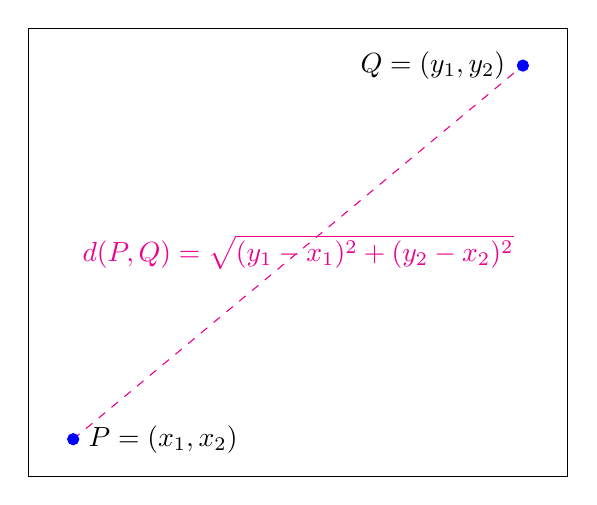
\begin{tikzpicture}
\begin{axis}[domain=0:3, xtick=\empty, ytick=\empty]
\addplot[blue, only marks] table{
1 1
2 2
};
\node[] () at (1.2,1) {\(P=(x_1,x_2)\)};
\node[] () at (1.8,2) {\(Q=(y_1,y_2)\)};
\draw[dashed, magenta] (1,1) -- (2,2)
node[midway]{\(d(P,Q)=\sqrt{(y_1-x_1)^{2}+(y_2-x_2)^{2}}\)};
\end{axis}
\end{tikzpicture}
\end{center}
Note that it carries the following properties which are natural for measuring
distance:
\begin{itemize}
\item \(d(P,Q)\ge 0\) for any points \(P,Q\in\R^{2}\), and \(d(P,Q)=0\) iff \(P=Q\)
\begin{intuition} Distance should be nonnegative. Also, given a point
\(\bullet\), the only point having \emph{zero} distance from (the same
``position'' as) \(\bullet\) is the point \(\bullet\) itself.
 \end{intuition}
\item \(d(P,Q)=d(Q,P)\) for any points \(P,Q\in\R^{2}\) \begin{intuition}
Distance between \(P\) and \(Q\) = distance between \(Q\) and \(P\).
\end{intuition}
\item (\emph{triangle inequality}) \(d(P,R)\le d(P,Q)+d(Q,R)\) for any points
\(P,Q,R\in\R^{2}\).
\begin{center}
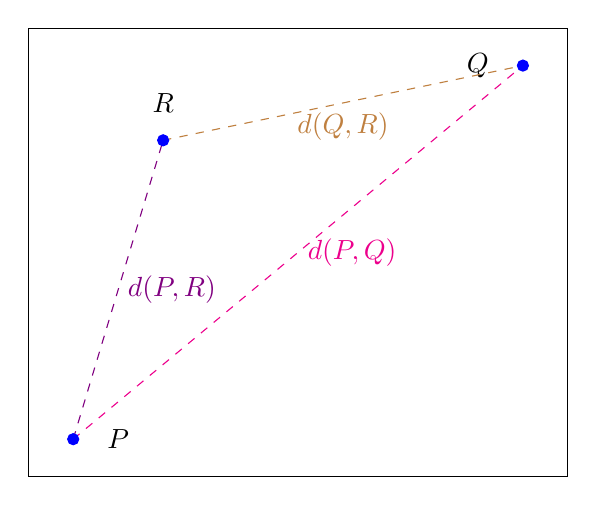
\begin{tikzpicture}
\begin{axis}[domain=0:3, xtick=\empty, ytick=\empty]
\addplot[blue, only marks] table{
1 1
2 2
1.2 1.8
};
\node[] () at (1.1,1) {\(P\)};
\node[] () at (1.9,2) {\(Q\)};
\node[] () at (1.2,1.9) {\(R\)};
\draw[dashed, magenta] (1,1) -- (2,2)
node[midway, right]{\(d(P,Q)\)};
\draw[dashed, violet] (1,1) -- (1.2,1.8)
node[midway, right]{\(d(P,R)\)};
\draw[dashed, brown] (1.2,1.8) -- (2,2)
node[midway, below]{\(d(Q,R)\)};
\end{axis}
\end{tikzpicture}
\end{center}
\end{itemize}
These properties define a \emph{metric}.
\item Let \(X\) be a nonempty set. Then, a \defn{metric} is a function
\(d:X\times X\to\R\) satisfying:
\begin{enumerate}[label={(M\arabic*)}]
\item For any \(x,y\in X\), \(d(x,y)\ge 0\) and \(d(x,y)=0\) iff \(x=y\).
\item For any \(x,y\in X\), \(d(x,y)=d(y,x)\).
\item For any \(x,y,z\in X\), \(d(x,z)\le d(x,y)+d(y,z)\).
\end{enumerate}
We also call the ordered pair \((X,d)\) a \defn{metric space}.

\begin{note}
When the choice of the metric \(d\) is clear from context, we may simply write
\(X\) instead of \((X,d)\). For example, unless stated otherwise, the metric
chosen when \(X=\R^n\) would the Euclidean distance.
\end{note}

This definition of metric space captures the idea of \emph{points} and
\emph{distances}. For any \(x,y\in X\), \(d(x,y)\) is the \defn{distance
between \(x\) and \(y\) with respect to \(d\)}. Elements in \(X\) are
\defn{points}.

\item Sometimes we only want to focus on a certain ``part'' of a metric space
(without altering the way of measuring distance). This leads to the notion of
\emph{metric subspace}. Let \((X,d)\) be a metric space and let \(Y\) be a
nonempty subset of \(X\). Define \(d_Y:Y\times  Y\to \R\) by
\[
d_Y(x,y)=d(x,y)
\]
for any \(x,y\in Y\). Then, \((Y,d_Y)\) is called a \defn{metric subspace} of
\((X,d)\) and \(d_Y\) is called as the \defn{relative metric inducted by \(d\)
on \(Y\)}. In fact, \((Y,d)\) is also a metric space.

\begin{pf}
Since \((X,d)\) is a metric space, (M1)--(M3) hold for all the points in \(X\).
Now, as \(Y\subseteq X\), every point in \(Y\) is also a point in \(X\), so
immediately (M1)--(M3) are satisfied for all the points in \(Y\) also.
\end{pf}
\end{enumerate}
\subsection{Examples of Metric Spaces}
\label{subsect:metric-sp-eg}
\begin{enumerate}
\item The definition of metric space is quite general. Indeed, many kinds of
sets (equipped with a certain metric \(d\)) can be metric spaces. We will give
some examples of metric spaces in \Cref{subsect:metric-sp-eg} (and \emph{prove}
that some are indeed metric spaces).

\item (a familiar one) Let \(X=\R^n\). For any points \(P=(x_1,\dotsc,x_n)\)
and \(Q=(y_1,\dotsc,y_n)\) in \(\R^n\), define
\(d(P,Q)=\sqrt{(y_1-x_1)^{2}+\dotsb+(y_n-x_n)^{2}}\) (Euclidean distance).
Then, \((X,d)\) is a metric space.

\begin{pf}
For (M1), \(d(P,Q)\ge 0\) follows from the nonnegativity of square root
function. Also, we have
\[
d(P,Q)=0\iff (y_1-x_1)^{2}+\dotsb+(y_n-x_n)^{2}=0
\iff \begin{cases}
y_1=x_1\\
y_2=x_2\\
\quad\;\vdots\\
y_n=x_n
\end{cases}
\iff
P=Q.
\]
(M2) follows from the property that \((y_i-x_i)^{2}=(x_i-y_i)^{2}\) for any
\(i=1,\dotsc,n\).

(M3) can be proven by using some algebraic tricks and Cauchy-Swartz inequality,
but we shall omit the details.
\end{pf}
\item Let \(X=S^2=\{(x,y,z):x^2+y^2+z^2=1\}\subseteq\R^3\), an unit sphere in
\(\R^3\).
\begin{center}
\begin{tikzpicture}
\draw[blue] (0,0) circle [radius=3cm];
\draw[blue] (-3,0) arc (180:360:3 and 0.6);
\draw[blue, dashed] (3,0) arc (0:180:3 and 0.6);
\node[violet, fill, circle, inner sep=0pt, minimum size=1.5mm] (start) at (0,-0.3) {};
\node[] () at (0.5,-0.3) {start};
\node[] () at (1.5,1.414) {end};
\node[brown, fill, circle, inner sep=0pt, minimum size=1.5mm] (end) at (1,1.414) {};
\draw[->, dashed, green!50!black] (start) .. controls (0.4, 0.25) .. (end);
\draw[->, dashed, red] (start) .. controls (-5.7,-6.95) and (3.7,5.95) .. (end);
\end{tikzpicture}
\end{center}
To motivate the definition of the following metric, suppose that the unit
sphere represents the ``Earth'' \faIcon{globe-americas}, and the two points
(\({\color{violet}\bullet}\) and \({\color{brown}\bullet}\)) on it represent
two places. Now, suppose that you want to travel \faIcon{plane} from
\({\color{violet}\bullet}\) to \({\color{brown}\bullet}\). Intuitively, the
shortest path for the travel is represented by the {\color{green!50!black}green
dashed arrows} (one cannot ``drill through the Earth straightly'' to go to
\({\color{brown}\bullet}\)!). It then appears that the arc length of that path
should be the distance between the two points.

Mathematically, we define \(d(x,y)=\) the length of the smaller arc on the
(unique) great circle (a planar circle on \(S^2\) with unit radius) joining the
two points \(x\) and \(y\). Then, \((X,d)\) is again a metric space.

\begin{pf}
Omitted.
\end{pf}
\item It turns out that one can form a metric space from \emph{any} set, using
the \emph{discrete metric}. Let \(X\) be any set. Then, for any \(x,y\in X\),
define
\[
d(x,y)=1-\delta_{xy}
\]
where \(\displaystyle \delta_{xy}=\begin{cases}
1&\text{if \(x=y\)};\\
0&\text{otherwise}.
\end{cases}
\) This metric is called \defn{discrete metric} (under which the distance
between two different points is \emph{always} one, and the distance between two
identical points are zero). \((X,d)\) is a metric space (sometimes called
\defn{discrete metric space}).

\begin{pf}
Fix any \(x,y\in X\). Then, since \(d(x,y)=0\text{ or }1\), it must be
nonnegative. Furthermore, we have \(d(x,y)=0\iff \delta_{xy}=1\iff x=y\), so
(M1) is satisfied.

(M2) follows from the fact that \(\delta_{xy}\) is symmetric (i.e.,
\(\delta_{xy}=\delta_{yx}\)).

For (M3), we prove by cases.
\begin{itemize}
\item Case 1: \(x=z\). Then, we have \(d(x,z)=0\le d(x,y)+d(y,z)\) (as RHS must
be nonnegative).
\item Case 2: \(x\ne z\). Then, \(d(x,z)=1\). Now, consider:
\begin{enumerate}
\item Subcase 1: \(x\ne y\). Then, \(d(x,y)+d(y,z)=(1+0)\text{ or }(1+1)\).
\item Subcase 2: \(z\ne y\). Then, \(d(x,y)+d(y,z)=(0+1)\text{ or }(1+1)\).
\end{enumerate}
In either subcase, we have \(d(x,y)+d(y,z)\ge 1=d(x,z)\), as desired.
\end{itemize}
\end{pf}
\item As mentioned earlier, MATH3401 is about studying continuous functions on
metric space. So, here we consider an example of a metric space for a set of
\emph{continuous functions}. Let \(X=C[a,b]\), the set of all (real-valued)
continuous functions with domain \([a,b]\). In this case, each ``point'' is
indeed a function (rather than a number or a vector). How should we measure the
distance between two \emph{functions}?

There are multiple ways to do so, but the following three are relatively more
famous. For any functions \(f,g\in X\):
\begin{itemize}
\item \textit{\(L^2\) norm:}
\[
d_2(f,g)=\qty[\int_{a}^{b}[f(x)-g(x)]^{2}\dd{x}]^{1/2}\triangleq\|f-g\|_{2}.
\]
\item \textit{\(L^1\) norm:}
\[
d_1(f,g)=\int_{a}^{b}|f(x)-g(x)|\dd{x}\triangleq\|f-g\|_{1}.
\]
\item \textit{\(L^{\infty}\) norm:}
\[
d_{\infty}(f,g)=\sup\{|f(x)-g(x)|:x\in[a,b]\}\triangleq\|f-g\|_{\infty}.
\]
\begin{note}
In general, for any \(p\ge 1\), we have the \emph{\(L^p\) norm}:
\[
d_p(f,g)=\qty[\int_{a}^{b}[f(x)-g(x)]^{p}\dd{x}]^{1/p}\triangleq\|f-g\|_{p}.
\]
It turns out that the limit of \(d_{p}(f,g)\) as \(p\to\infty\) is
\(\sup\{|f(x)-g(x)|:x\in[a,b]\}\), hence the name ``\(L^\infty\) norm''.
\end{note}

\begin{intuition}
\(L^1\) and \(L^2\) norms capture the intuitive idea that two functions \(f\)
and \(g\) are ``close'' if for ``most'' input \(x\), \(f(x)\) and \(g(x)\) are
``close''.
\end{intuition}
\end{itemize}
\begin{pf}

\end{pf}
\item The last example we give here concerns a metric space with \emph{finite}
set. Let \(X=\{a,b,c\}\) (where \(a\), \(b\), and \(c\) are distinct). Define
the function \(d:X\times X\to\R\) by
\begin{center}
\begin{tabular}{c|ccc}
\toprule
\(d\)&\(a\)&\(b\)&\(c\)\\
\midrule
\(a\)&0&2&3\\
\(b\)&2&0&2\\
\(c\)&3&2&0\\
\bottomrule
\end{tabular}
\end{center}
Then, \((X,d)\) is a metric space.

\begin{pf}
(M1) follows since every entry in the table is nonnegative and all the
diagonal entries are zero. (M2) follows since the table is symmetric along its
diagonal.

For (M3), we can exhaust all the possibilities (since there are only finitely
many possible pairs of points) and verify it.
\end{pf}
\end{enumerate}
\subsection{Distance Between a Point and a Set}
\begin{enumerate}
\item Apart from distance between two points, sometimes we are interested in
knowing distance between a point and a set. How should we define it?
\begin{center}
\begin{tikzpicture}
\draw[fill, blue] (0,0) circle [radius=0.5mm];
\draw[fill, magenta!20!white] (-5,0) ellipse [x radius=2cm, y radius=1cm];
\node[] (set) at (-5,0) {\(S\)};
\node[] (pt) at (0,-0.5) {\(P\)};
\draw[-Latex] (-2.5,-2) -- (set);
\draw[-Latex] (-2.5,-2) -- (pt);
\node[] () at (-2.5,-2.5) {distance?};
\end{tikzpicture}
\end{center}

\item An intuitive way to measure the distance between the point \(P\) and the
set \(S\) is to use the length of the ``\emph{shortest}'' path for ``travelling''
from point \(P\) (``your current location'') to set \(S\) (``island'').
\begin{center}
\begin{tikzpicture}
\draw[fill, magenta!20!white] (-5,0) ellipse [x radius=2cm, y radius=1cm];
\node[] (set) at (-5,0) {\(S\)};
\node[] () at (-6,0.6) {\faIcon{tree}};
\node[] () at (-6,-0.5) {\faIcon{tree}};
\node[] () at (-4.5,-0.3) {\faIcon{tree}};
\node[] () at (-5.5,0.4) {\faIcon{tree}};
\node[] (pt) at (0,-0.5) {\(P\)};
\node[] () at (0,0) {\faIcon{swimmer}};
\draw[fill, blue] (0,0) circle [radius=0.5mm];
\draw[-Latex, dashed, green!50!black] (0,0) -- (-3,0)
node[midway, above]{shortest};
\draw[-Latex, dashed, red, opacity=0.5] (0,0) -- (-3.5,-0.6614);
\draw[-Latex, dashed, red, opacity=0.5] (0,0) -- (-4,0.86603);
\end{tikzpicture}
\end{center}
\item Mathematically, in a metric space \((X,d)\), given any point \(P\in X\)
and any nonempty set \(S\subseteq X\), the \defn{distance from point \(P\) to
set \(S\)} is
\[
d(P,S)=\inf_{x\in S}\{d(P,x)\}.
\]
\begin{note}
The notation \(\displaystyle \inf_{x\in S}\{d(P,x)\}\) is another way to write \(\inf\{d(P,x):x\in S\}\).
\end{note}
\item Now, after ``arriving'' the set \(S\) (``island''), we may start
``exploring'' \faIcon{search} it. We would then like to know how ``large'' the
``island'' is.
\begin{center}
\begin{tikzpicture}
\draw[fill, magenta!20!white] (-5,0) ellipse [x radius=2cm, y radius=1cm];
\node[] (set) at (-5,0) {\(S\)};
\node[] () at (-6,0.6) {\faIcon{tree}};
\node[] () at (-6,-0.5) {\faIcon{tree}};
\node[] () at (-4.5,-0.3) {\faIcon{tree}};
\node[] () at (-5.5,0.4) {\faIcon{tree}};
\node[] () at (-3,0) {\faIcon{child}};
\end{tikzpicture}
\end{center}
\item Recall the notion of \emph{diameter} for a circle. It is the length of a
line segment passing through the center and whose endpoints lie on the circle.
It is also the \emph{maximum distance} between two points lying on the circle.
\begin{center}
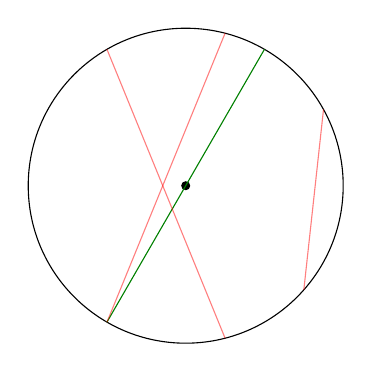
\begin{tikzpicture}
\draw[] (0,0) circle [radius=2cm];
\draw[fill] (0,0) circle [radius=0.5mm];
\draw[green!50!black] (-1,-1.732) -- (1,1.732);
\draw[red, opacity=0.5] (-1,-1.732) -- (0.5,1.936);
\draw[red, opacity=0.5] (1.5,-1.323) -- (1.75,0.9682);
\draw[red, opacity=0.5] (-1,1.732) -- (0.5,-1.936);
\end{tikzpicture}
\end{center}
In a similar manner, we may define the notion of \emph{diameter} for other
kinds of geometrical objects as follows.

Let \((X,d)\) be a metric space. For any nonempty set \(S\subseteq X\), the
\defn{diameter} of \(S\) is
\[
D(S)=\sup_{P,Q\in S}\{d(P,Q)\}.
\]
\item Examples: Consider the metric space \(\R\) (equipped with Euclidean
distance). Then:
\begin{itemize}
\item the diameter of the closed interval \([0,1]\) is \(1\)
\item the diameter of the open interval \((0,1)\) is \(1\) \begin{note}
If we use ``\(\max\)'' instead of ``\(\sup\)'' in the definition for diameter,
then this is \emph{undefined}, which is unsatisfactory. Hence, in the
definition we use the notion of supremum instead of maximum.
\end{note}
\end{itemize}
\end{enumerate}
\subsection{Topology of Metric Spaces}
\begin{enumerate}
\item Roughly speaking, \emph{topology} studies the properties of a geometric
object that are preserved under ``continuous deformations''. Here, we will
introduce some important notions related to metric space topology.

\item For the case of \(\R\), we are familiar with the notions of \emph{open
interval} (not including its endpoints) and \emph{closed interval} (including
its endpoints). We can generalize these notions to \emph{open sets} and
\emph{closed sets} respectively, which are fundamental to metric space
topology.

\item To define open and closed sets, we need to introduce some preliminary
notions. Consider a metric space \((X,d)\) throughout. Let \(a\in X\) and
\(r>0\) (a real number). Then, the \defn{open ball in \(X\) with center \(a\)
and radius \(r\)} is
\[
B(a,r)=\{x\in X: d(a,x)\vc{<}r\},
\]
and the \defn{closed ball in \(X\) with center \(a\) and radius \(r\)} is
\[
\overline{B}(a,r)=\{x\in X: d(a,x)\vc{\le}r\},
\]
\begin{center}
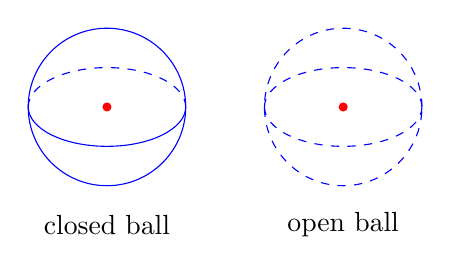
\begin{tikzpicture}
\draw[blue] (0,0) circle [radius=1cm];
\draw[blue] (-1,0) arc (180:360:1 and 0.5);
\draw[blue, dashed] (1,0) arc (0:180:1 and 0.5);
\draw[red, fill] (0,0) circle [radius=0.5mm];
\node[] () at (0,-1.5) {closed ball};

\draw[blue, dashed] (3,0) circle [radius=1cm];
\draw[blue, dashed] (2,0) arc (180:360:1 and 0.5);
\draw[blue, dashed] (4,0) arc (0:180:1 and 0.5);
\draw[red, fill] (3,0) circle [radius=0.5mm];
\node[] () at (3,-1.5) {open ball};
\end{tikzpicture}
\end{center}
\begin{note}
Let \(S\) be a nonempty subset of \(X\).  Considering \((S,d)\) as a metric
subspace of \((X,d)\) (which is itself a metric space), an open ball in \(S\)
with center \(a\) and radius \(r\) can be expressed as
\[
B_{S}(a,r)=\{x\in S:d(a,x)<r\}=B_{X}(a,r)\cap S
\]
where \(B_X(a,r)\) is the open ball with same center and radius, but in \(X\).
\end{note}
\item Let \(S\subseteq X\). Then, a point \(a\in S\) is an \defn{interior point
of \(S\)} if there exists \(r>0\) such that
\[
B(a,r)\subseteq S.
\]
The \defn{interior of \(S\)}, denoted by \(S^{\circ}\) or
\(\operatorname{int}S\), is the set of all interior points of \(S\).

\begin{intuition}
Viewing \(S\) as an ``island'', an interior point of \(S\) is a location at the
``inner part'' of ``island'', and the interior of \(S\) is the whole ``inner
part'' of ``island''.
\end{intuition}

\begin{center}
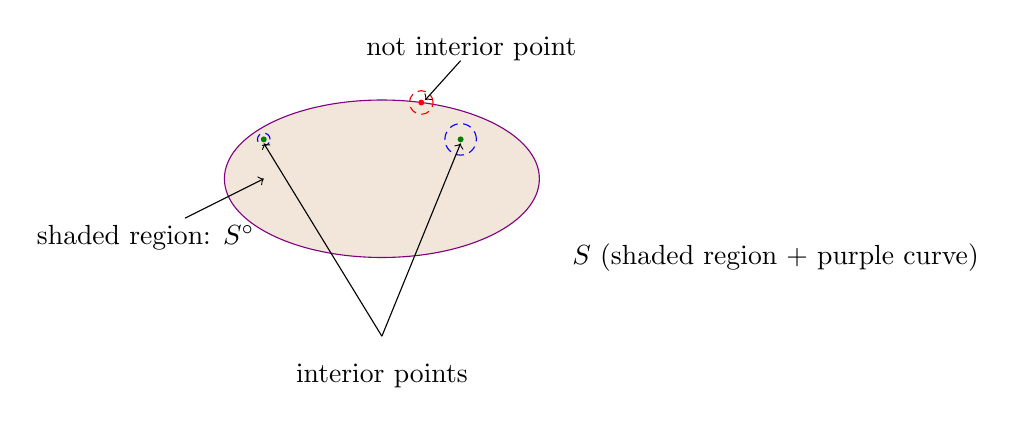
\begin{tikzpicture}
\draw[fill, brown!20!white, draw=violet] (0,0) ellipse [x radius=2cm, y radius=1cm];
\draw[fill, green!50!black] (1,0.5) circle [radius=0.3mm];
\draw[draw, densely dashed, blue] (1,0.5) circle [radius=2mm];
\draw[fill, green!50!black] (-1.5,0.5) circle [radius=0.3mm];
\draw[draw, densely dashed, blue] (-1.5,0.5) circle [radius=0.8mm];
\draw[fill, red] (0.5,0.9682) circle [radius=0.3mm];
\draw[draw, densely dashed, red] (0.5,0.9682) circle [radius=1.5mm];
\draw[->] (1,1.5) -- (0.55,1)
node[pos=-0.3]{not interior point};
\draw[->] (0,-2) -- (-1.5,0.45);
\draw[->] (0,-2) -- (1,0.45);
\node[] () at (0,-2.5) {interior points};
\node[] () at (5,-1) {\(S\) (shaded region + purple curve)};
\draw[->] (-2.5,-0.5) -- (-1.5,0)
node[pos=-0.5]{shaded region: \(S^{\circ}\)};
\end{tikzpicture}
\end{center}

\item Now we are ready to define open and closed sets. A set \(S\subseteq X\)
is \defn{open in \(X\)} if \(S=S^{\circ}\), and it is \defn{closed in \(X\)} if
\(X\setminus S\) is open in \(X\).
\begin{center}
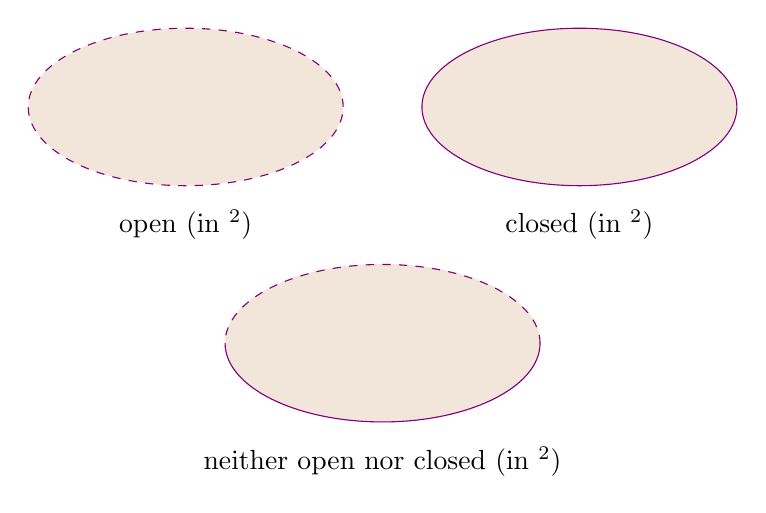
\begin{tikzpicture}
\draw[fill, brown!20!white, draw=violet, dashed] (0,0) ellipse [x radius=2cm, y radius=1cm];
\node[] () at (0,-1.5) {open (in \(\R^2\))};
\draw[fill, brown!20!white, draw=violet] (5,0) ellipse [x radius=2cm, y radius=1cm];
\node[] () at (5,-1.5) {closed (in \(\R^2\))};
\draw[fill, brown!20!white] (2.5,-3) ellipse [x radius=2cm, y radius=1cm];
\draw[violet, dashed] (4.5,-3) arc (0:180:2 and 1);
\draw[violet] (0.5,-3) arc (180:360:2 and 1);
\node[] () at (2.5,-4.5) {neither open nor closed (in \(\R^2\))};
\end{tikzpicture}
\end{center}
\begin{remark}
\item When the set \(S\) is empty, there is no interior point of \(S\) (since \(S\)
does not even have element!). Thus, the interior of \(S\) is empty as well.
Hence, we have \(S=S^{\circ}=\varnothing\), meaning that empty set is open in
\(X\). (This holds true for any metric space \((X,d)\)!)

\item We always have \(S\supseteq S^{\circ}\) since every interior point of
\(S\) must be an element of \(S\) (by definition). Hence, to show that a set
\(S\) is open in \(X\), it suffices to show that \(S\subseteq S^{\circ}\),
i.e., every point in \(S\) is an interior point of \(S\).

\item The concepts of ``open'' and ``closed'' are with respect to the set \(X\)
in the metric space, so we need to specify what set \(X\) we are referring to
when talking about open and closed sets (unless it is clear from context).
\end{remark}
\item The concepts of open and closed sets are not mutually exclusive. Indeed,
a set can be \emph{both open and closed}.
\begin{proposition}
\label{prp:both-open-and-closed}
Let \((X,d)\) be a metric space. Then, \(\varnothing\) and \(X\) are both open
and closed in \(X\).
\end{proposition}
\begin{pf}
Firstly, from the remark above we know that \(\varnothing\) is open in \(X\).
Now we will show that \(X\) is also open in \(X\). Consider any point \(a\in
X\), and choose any \(r>0\). Then, we immediately have
\[
B(a,r)=\{x\vc{\in X}:d(a,x)<r\}\vc{\subseteq X},
\]
meaning that the point \(a\) is an interior point of \(X\). Thus, we have
\(X\subseteq X^{\circ}\) (which implies that \(X=X^{\circ}\)) and hence \(X\)
is open in \(X\).

Next, note that \(\varnothing=X\setminus \blc{X}\) and
\(X=X\setminus\brc{\varnothing}\) are open in \(X\). Thus, \(\blc{X}\) and
\(\brc{\varnothing}\) are closed in \(X\).
\end{pf}

\item For different metric spaces, the same set can have different properties
regarding openness and closedness. The following example illustrates this
phenomenon.

Let \(X=\R\) and equip it with the Euclidean distance metric \(d\) (defined by
\(d(x,y)=|x-y|\) for any \(x,y\in X\)). Let \(Y=[0,1)\cup (2,3)\subseteq X\),
which induces a metric subspace of \((X,d)\): \((Y,d_{Y}\)). Then, \(S=[0,1)\)
is neither open nor closed in \(X\), but is both open and closed in \(Y\).

\begin{pf}
Firstly, \(S=[0,1)\) is not open in \(X\) since \(0\in S\) is \emph{not} an
interior point of \(S\) (for any \(r>0\), the open ball \(B(0,r)\) contains
elements outside \(S\)). It is also not closed in \(X\) since \(X\setminus
S=(-\infty,0)\cup[1,\infty)\) is not open in \(X\) (we can similarly show that
\(1\) is not an interior point of \(X\setminus S\)). This shows \(S\) is
neither open nor closed in \(X\).
\begin{center}
\begin{tikzpicture}
\draw[-Latex] (0,0) -- (10,0);
\node[] () at (3,0) {[};
\node[] () at (7,0) {)};
\node[] () at (3,-0.5) {\(0\)};
\node[] () at (7,-0.5) {\(1\)};
\node[blue] () at (2.8,0) {(};
\node[blue] () at (3.2,0) {)};
\draw[line width=0.1cm, opacity=0.5, red, line cap=round] (2.8,0) -- (2.93,0);
\draw[red, ->] (2,-1) -- (2.85,-0.2)
node[pos=-0.3]{outside \(S\)!};
\end{tikzpicture}
\end{center}

Next, we will prove that \(S\) is both open and closed in \(Y\). For the
openness, we will only show that \(0\) is an interior point of \(Y\). (Every
other point in \(S\) is clearly an interior point of \(Y\), by choosing
a sufficiently small \(r>0\) (e.g., \(\displaystyle
r=\frac{1}{2}\cdot \max\{\text{distance between the point and \(0\)}, \text{distance
between the point and \(1\)}\}\)).)

We first need to choose a small \(r>0\), say \(r=0.1\). Then, we have
\[
B(0,r)=\{y\in\vc{Y}:|y-0|<r\}
=\{y\in\vc{[0, 1)\cup (2,3)}:y<0.1\}
=[0,0.1)\subseteq Y
\]
(which is \underline{not} \((-0.1,0.1)\) \warn{}). Thus, \(0\) is an interior
point of \(Y\), and hence \(S\) is open in \(Y\).
\begin{center}
\begin{tikzpicture}
\draw[-Latex] (0,0) -- (10,0);
\node[] () at (3,0) {[};
\node[] () at (7,0) {)};
\node[] () at (3,-0.5) {\(0\)};
\node[] () at (7,-0.5) {\(1\)};
\node[blue] () at (3,0) {[};
\node[blue] () at (3.2,0) {)};
\draw[violet, ->] (3.5,-1) -- (3.1,-0.2)
node[pos=-0.3]{altered ``shape'' of \(B(0,r)\)};
\end{tikzpicture}
\end{center}
For the closedness, note that \(Y\setminus S=(2,3)\). Every point in
\(Y\setminus S\) can be shown to be an interior point of \(Y\) (by choosing a
sufficient small \(r>0\), like what was mentioned above). So, \(Y\setminus S\)
is open in \(Y\), thus \(S\) is closed in \(Y\).
\end{pf}
\end{enumerate}
